% ============================================================
%  Req2UI - Graduation Thesis
%  From Natural Language to Secure Software Artifacts Using AI
%  Arab Academy for Science, Technology, and Maritime Transport
%  Compile on Overleaf (pdfLaTeX) or locally with: latexmk -pdf main.tex
% ============================================================
\documentclass[12pt,a4paper,oneside]{report}

\usepackage[utf8]{inputenc}
\usepackage[T1]{fontenc}
\usepackage{lmodern}
\usepackage[margin=1in]{geometry}
\usepackage{graphicx}
\graphicspath{{figures/}}
\usepackage{booktabs}
\usepackage{longtable}
\usepackage{array}
\usepackage{tabularx}
\usepackage{xcolor}
\usepackage{enumitem}
\usepackage{caption}
\usepackage{titlesec}
\usepackage{setspace}
\usepackage{fancyhdr}
\usepackage[hidelinks]{hyperref}

\definecolor{accent}{HTML}{2F5C8F}
\captionsetup{font=small,labelfont=bf}
\onehalfspacing

% Header / footer
\pagestyle{fancy}
\fancyhf{}
\fancyhead[L]{\small\itshape Req2UI}
\fancyhead[R]{\small\thepage}
\renewcommand{\headrulewidth}{0.4pt}

% Helper column types
\newcolumntype{L}[1]{>{\raggedright\arraybackslash}p{#1}}

% Requirement table helper
\newenvironment{reqtable}[1]{%
  \begin{longtable}{L{1.6cm} L{4.2cm} L{2cm} L{6cm}}
  \caption{#1}\\
  \toprule
  \textbf{ID} & \textbf{Requirement} & \textbf{Priority} & \textbf{Description} \\
  \midrule
  \endfirsthead
  \toprule
  \textbf{ID} & \textbf{Requirement} & \textbf{Priority} & \textbf{Description} \\
  \midrule
  \endhead
  \bottomrule
  \endfoot
}{%
  \end{longtable}
}

% ============================================================
\begin{document}

% ----------------------- TITLE PAGE -----------------------
\begin{titlepage}
\centering
\vspace*{0.5cm}

\includegraphics[width=3.2cm]{aast-logo.png}\\[0.6cm]
{\large Arab Academy for Science, Technology, and Maritime Transport\\
College of Computing and Information Technology\\
Smart Village\par}
\vspace{2cm}
{\Huge\bfseries Req2UI: From Natural Language to Secure Software Artifacts Using AI\par}
\vspace{0.6cm}
{\Large Graduation Project\par}
\vspace{2cm}
{\large A Thesis submitted in partial fulfillment of the requirements\\
of B.Sc. in ``Software Engineering.''\par}
\vspace{1.5cm}
{\large by\par}
\vspace{0.3cm}
{\large
Mennatallah Hany Mohamed\\
Mayar Hany Mohamed\\
Yasmin Haitham Shaheen\\
Malak Tarek Tolba\\
Mohamed Bassem\par}
\vspace{1.5cm}
{\large Supervised By\\[0.2cm]
Dr. Salma Radwan Abdel-Hamid\par}
\vfill
{\large Smart Village, Cairo, 2025--2026\par}
\end{titlepage}

% ----------------------- FRONT MATTER -----------------------
\pagenumbering{roman}

\chapter*{Abstract}
\addcontentsline{toc}{chapter}{Abstract}
The project aims to develop an AI-driven Automated Software Requirement Specification (SRS) Generator that streamlines the process of requirement gathering and documentation. The system automatically generates functional, non-functional, and security requirements based on project inputs. It identifies sensitive features such as login systems, payment gateways, or data uploads and integrates related security policies automatically. Additionally, the system converts generated requirements into low-fidelity UI prototypes using HTML/Tailwind templates. These prototypes visually represent the application's key functional and security components, including authentication and privacy features. Finally, the project integrates an automated test case generator that creates functional and security test cases aligned with OWASP Top 10 guidelines. This approach ensures that security and quality are embedded early in the software development lifecycle, reducing development time and enhancing software reliability.

\chapter*{Acknowledgment}
\addcontentsline{toc}{chapter}{Acknowledgment}
We would like to express our sincere gratitude to everyone who contributed to the successful completion of this graduation project.

First and foremost, we would like to thank our supervisor, Dr. Salma Radwan Abdel-Hamid, for her continuous guidance, valuable feedback, and constant support throughout all stages of this project. Her academic insight and encouragement were essential in shaping the direction and quality of this work.

We would also like to extend our appreciation to the Arab Academy for Science, Technology, and Maritime Transport (AASTMT), College of Computing and Information Technology -- Smart Village, for providing the academic environment, resources, and facilities necessary to conduct this project.

Special thanks go to our families and friends for their continuous support, patience, and motivation during the development of this project. Finally, we would like to thank everyone who contributed directly or indirectly to the completion of this work.

\tableofcontents
\listoffigures
\listoftables

% ----------------------- ABBREVIATIONS -----------------------
\chapter*{Abbreviations}
\addcontentsline{toc}{chapter}{Abbreviations}
\begin{longtable}{L{3cm} L{10cm}}
\toprule
\textbf{Abbreviation} & \textbf{Description} \\
\midrule
\endhead
AI & Artificial Intelligence \\
API & Application Programming Interface \\
ASVS & Application Security Verification Standard \\
CI/CD & Continuous Integration / Continuous Deployment \\
CRUD & Create, Read, Update, Delete \\
GUI & Graphical User Interface \\
HTML & HyperText Markup Language \\
IEEE & Institute of Electrical and Electronics Engineers \\
JSON & JavaScript Object Notation \\
JWT & JSON Web Token \\
LLM & Large Language Model \\
NLP & Natural Language Processing \\
NFR & Non-Functional Requirement \\
OWASP & Open Web Application Security Project \\
PDF & Portable Document Format \\
REST & Representational State Transfer \\
SDLC & Software Development Life Cycle \\
SRS & Software Requirements Specification \\
SSE & Server-Sent Events \\
UI & User Interface \\
UML & Unified Modeling Language \\
UX & User Experience \\
\bottomrule
\caption{Abbreviations}
\end{longtable}

% ----------------------- MAIN MATTER -----------------------
\clearpage
\pagenumbering{arabic}

% ============================================================
\chapter{Introduction}
Modern software engineering relies heavily on accurate, complete, and well-structured documentation. Among these documents, the Software Requirements Specification (SRS) plays a critical role as it defines the functional, non-functional, and security requirements that guide the entire development lifecycle. However, creating an SRS manually is often time-consuming, inconsistent, and prone to human error---especially for teams with limited experience in requirements engineering. With the rapid growth of Artificial Intelligence (AI) and automation tools, new opportunities have emerged to streamline and enhance this phase of software development.

This project introduces an AI-powered Automated SRS Generator that transforms a user's natural-language description of a system into a complete SRS document, including functional requirements, non-functional requirements, and security requirements following OWASP standards. In addition, the system automatically generates UI prototypes and functional and security test cases, providing an integrated, end-to-end solution for early-stage software design. By combining Natural Language Processing (NLP), automated UI generation, and test automation, the proposed system aims to reduce development time, improve requirement accuracy, and support secure-by-design principles from the very beginning of the software development lifecycle.

\section{Motivation}
In modern software development, writing Software Requirement Specifications (SRS) is a time-consuming and error-prone process. Many teams still rely on manual documentation, leading to inconsistencies, unclear requirements, and security oversights. With the rise of AI-driven tools, there is an opportunity to automate this process---not only to save time but also to embed security and testing awareness early in the development lifecycle. This project aims to reduce documentation effort, improve requirement quality, and promote secure-by-design software engineering by automatically generating SRS, UI prototypes, and test cases.

\section{Problem Statement}
The current challenge in software engineering lies in the manual, repetitive, and unstructured nature of requirement gathering and documentation. Traditional tools such as IBM Rational RequisitePro or Microsoft Word depend heavily on human input, which increases the risk of missing functional or security requirements. Furthermore, the lack of integration between requirements, UI design, and testing results in inconsistencies and delays in development. This project addresses these issues by developing an AI-driven automated SRS generator that can produce functional, non-functional, and security requirements, generate visual UI prototypes, and automatically create test cases aligned with OWASP Top 10 security guidelines.

\section{Objectives}
\begin{itemize}[leftmargin=*]
  \item To design and implement an AI-based system capable of generating complete SRS documents automatically.
  \item To integrate security requirement generation into the SRS process based on project context and OWASP standards.
  \item To develop a UI prototype generator using HTML/Tailwind templates that reflects key functional and security components.
  \item To implement an automated test case generator for both functional and security test cases.
  \item To ensure that the overall system promotes secure-by-design development and reduces the manual workload for developers.
\end{itemize}

\section{Problem Complexity}
\begin{itemize}[leftmargin=*]
  \item The need for accurate natural language understanding to extract requirements from user input.
  \item Integrating multiple technologies---AI/NLP models, OWASP rules, and testing frameworks---in one pipeline.
  \item Balancing creativity (AI-generated text) with structure (SRS templates).
  \item Automatically linking generated requirements to corresponding UI elements and test cases in a consistent and logical way.
  \item Managing the dynamic nature of security rules, which evolve over time with new vulnerabilities and standards.
\end{itemize}

\section{Constraints}
The proposed Automated SRS Generator is subject to a set of realistic project constraints that limit the scope and implementation of the system. These constraints are aligned with the defined non-functional requirements and the academic nature of the project.

\begin{longtable}{L{3.5cm} L{9.5cm}}
\caption{System constraints}\\
\toprule
\textbf{Constraint Type} & \textbf{Description} \\
\midrule
\endhead
Deadline Constraint & The project must be completed within the academic timeline defined by the graduation project schedule. All development, testing, and documentation activities are limited to the assigned semester duration. \\
Budget Constraint & The project is developed with zero or minimal financial cost. Usage of paid services such as AI APIs is limited to free tiers or educational credits, which restricts extensive experimentation or large-scale deployment. \\
Software Constraint & The system is constrained to deliver fast and reliable performance by generating complete SRS documents within acceptable response times and supporting multiple concurrent users without noticeable degradation. It must ensure high usability and accessibility, comply with recognized accessibility standards, maintain high availability, automatically recover from errors, and preserve data integrity. Strong security constraints apply, including secure session management, input validation, and protection of all user data through modern encryption for both storage and transmission. \\
Hardware Constraint & Development and testing are performed on standard personal computers. The system is not designed to support high-performance computing environments or large-scale concurrent usage due to hardware limitations. \\
\bottomrule
\end{longtable}

\section{Standards}
This project is written according to the IEEE 12207 standard, which specifies requirements-specification standards (IEEE 830, shown in Chapter 4), UML, design standards, software process models, implementation standards, and testing standards (IEEE 829, shown in Chapter 7).

\begin{longtable}{L{6.5cm} L{6.5cm}}
\caption{Standards}\\
\toprule
\textbf{Standard} & \textbf{Reference in the Document} \\
\midrule
\endhead
IEEE 12207: Software Life Cycle Processes & Referenced throughout the document \\
IEEE 830: Software Requirements and Specification & Chapter 4 \\
IEEE 829: Testing & Chapter 7 \\
UML & Chapter 4 and Chapter 5 \\
OWASP (implementation standard) & Chapter 6 \\
\bottomrule
\end{longtable}

\section{Business Canvas}
\begin{longtable}{L{4cm} L{9cm}}
\caption{Business model}\\
\toprule
\textbf{Block} & \textbf{Description} \\
\midrule
\endhead
Value Proposition & Automated SRS generation, UI prototypes, functional \& security test cases, reduced time \& errors \\
Customer Segments & Software developers, students, startups, freelancers, academic institutions \\
Channels & Web application, online platform, institutional access \\
Customer Relationships & Self-service portal, documentation, automated support \\
Key Activities & AI processing, requirements generation, UI prototype creation, test case automation \\
Key Resources & Groq API, Google Gemini API, OWASP knowledge base, cloud hosting \\
Key Partners & AI providers, security tooling communities, cloud platforms (Vercel, Render, Neon) \\
Cost Structure & API usage costs, cloud hosting, maintenance, development time \\
Revenue Streams & Subscription plans, pay-per-use, enterprise licensing \\
\bottomrule
\end{longtable}

\section{Stakeholders}
\subsection{End User (Primary Stakeholder)}
End Users are the main beneficiaries of the system. They include software developers, students, startups, and freelancers who rely on the system to automatically generate software engineering artifacts. End Users interact with the system through a web-based interface to submit project descriptions, review generated outputs, and export results.

\noindent\textbf{Goals and Interests:} quickly generate structured SRS documents; visualize UI prototypes; obtain functional and security test cases; export software artifacts for further development.

\noindent\textbf{System Interactions (Use Cases):} Register / Login, Create Project, View SRS, View UI Prototype, View Test Cases, Export Artifacts.

\subsection{System Administrator (Secondary Stakeholder)}
The System Administrator is responsible for managing and maintaining the system's operational integrity. This stakeholder ensures system availability, monitors usage, and manages user accounts. Administrative functionality is primarily focused on system-level maintenance rather than direct artifact generation.

\noindent\textbf{Goals and Interests:} ensure system stability and availability; monitor usage and performance; manage user accounts and permissions; maintain system configuration.

\subsection{AI and Supporting Services}
AI and supporting services represent internal system components that enable intelligent automation. These services are invoked as internal subsystems responsible for processing user input and generating software artifacts. They include the large language model providers (Groq and Google Gemini) and the OWASP security knowledge base, and operate transparently in the background through \texttt{<<include>>} and \texttt{<<extend>>} relationships from End User use cases.

\section{Thesis Organization}
\begin{description}[leftmargin=*]
  \item[Chapter 1 -- Introduction:] presents an overview of the project, including the motivation, problem statement, objectives, scope, constraints, and standards.
  \item[Chapter 2 -- Background:] covers the theoretical foundations: SRS, automation in software engineering, AI in requirements engineering, test automation, and security within the SDLC.
  \item[Chapter 3 -- Related Work and Similar Systems:] reviews existing academic research and commercial tools, compares them, and identifies the research gap.
  \item[Chapter 4 -- Analysis:] presents the system overview, functional, non-functional, and security requirements.
  \item[Chapter 5 -- Design:] describes the system architecture, UML diagrams, technologies, and prototype.
  \item[Chapter 6 -- Implementation:] explains the implementation environment, technologies, and results.
  \item[Chapter 7 -- Testing:] presents the testing methodology and results.
  \item[Chapter 8 -- Conclusion and Future Work:] summarizes contributions and proposes future enhancements.
\end{description}

% ============================================================
\chapter{Background}
This chapter presents a comprehensive background of the key theoretical and technical concepts that underpin the proposed system. It discusses Software Requirements Specification (SRS), automation in software engineering, Artificial Intelligence (AI) in requirements engineering, test automation, and secure Software Development Life Cycle (SDLC) practices.

\section{Overview of Software Requirements Specification (SRS)}
A Software Requirements Specification (SRS) is a core artifact in software engineering that formally describes what a software system is expected to do and the constraints under which it must operate. Since the proposed project focuses on automatically generating SRS documents from natural-language input, a clear understanding of SRS concepts, structure, and challenges is essential.

\subsection{Definition of Software Requirements Specification}
An SRS is a structured and formal document that captures the complete set of functional requirements, non-functional requirements, and security requirements of a software system. Functional requirements describe the services and behaviors the system must provide, while non-functional requirements define quality attributes such as performance, usability, reliability, and scalability. Security requirements specify controls and safeguards needed to protect the system from potential threats. The SRS serves as a single source of truth for all stakeholders.

\subsection{Importance of SRS in the Software Development Life Cycle}
The SRS plays a critical role across all phases of the SDLC. During planning and analysis, it helps stakeholders agree on system scope, objectives, and constraints. In design and implementation, it guides architectural decisions and coding. During testing and validation, it acts as a baseline for creating test cases. Finally, during maintenance, it supports system evolution by enabling traceability between requirements, code, and tests.

\subsection{Challenges in Manual SRS Development}
Despite its importance, manual SRS development is prone to several challenges. Requirements are often written in natural language, which can lead to ambiguity, vagueness, and inconsistent interpretation. Incomplete requirements, conflicting statements, and lack of standardization are common issues. Additionally, security requirements are frequently under-specified or omitted, increasing the risk of vulnerabilities later in the SDLC.

\section{Automation in Software Engineering}
Automation has become a fundamental aspect of modern software engineering, aiming to reduce manual effort, improve productivity, and enhance process reliability.

\subsection{Role and Benefits of Automation}
Automation is widely applied throughout the SDLC, including requirements management, development, testing, deployment, and maintenance. Automated tools enable consistent documentation, faster execution of development tasks, and repeatable processes. The benefits include reduced human error, faster development cycles, improved accuracy, and enhanced software quality.

\subsection{Relevance of Automation to the Proposed System}
In the proposed system, natural-language user input is automatically transformed into structured SRS sections; UI prototypes are generated automatically to provide early visualization; and functional and security test cases are produced directly from the generated requirements. This integrated automation addresses the inefficiencies of traditional manual processes.

\section{Artificial Intelligence in Requirements Engineering}
AI has increasingly been adopted in requirements engineering to address the complexity and limitations of manual requirement analysis. AI techniques, particularly NLP and large language models, enable systems to interpret unstructured textual input and transform it into structured representations.

\subsection{Role and Advantages of AI in Requirements Engineering}
AI-based approaches allow automated analysis of stakeholder requirements expressed in natural language. NLP techniques can identify key entities, actions, constraints, and quality attributes. Large Language Models (LLMs) further enhance this capability by understanding contextual relationships and generating coherent, standardized requirement statements, reducing ambiguity and improving completeness.

\subsection{Use of AI in the Proposed System}
The proposed system leverages AI to automatically extract functional, non-functional, and security requirements from user-provided descriptions. It identifies security-sensitive components such as authentication, data storage, and access control, generates structured SRS documents, and derives corresponding test cases.

\section{Test Automation}
\subsection{Overview of Test Automation}
Automated testing replaces or supplements manual testing by executing predefined test scripts to validate system behavior. It is particularly effective for regression testing, performance testing, and repetitive validation tasks, offering faster execution, higher repeatability, and reduced human error.

\subsection{Relevance of Test Automation to the Proposed System}
In the proposed system, test automation is tightly integrated with requirements generation. Functional test cases and OWASP-aligned security test cases are automatically generated from the SRS, ensuring early test coverage and supporting a secure-by-design approach.

\subsection{Benefits of Test Automation}
Test automation provides rapid feedback to developers, improves defect detection, supports continuous integration, enhances software quality, and ensures consistent validation throughout the SDLC.

\section{Security in the Software Development Life Cycle}
\subsection{Importance of Secure SDLC}
A secure SDLC incorporates security considerations during requirements analysis, design, implementation, testing, deployment, and maintenance. Defining security requirements early ensures that architectural and design decisions account for potential threats.

\subsection{Relevance of Secure SDLC to the Proposed System}
The proposed system embeds security from the requirements stage by automatically detecting security-sensitive features and generating security requirements and OWASP Top 10--aligned test cases.

\subsection{Benefits of Integrating Security Early}
Early integration of security practices results in more robust and resilient systems, fewer vulnerabilities, lower remediation costs, and improved compliance with security standards and regulations.

% ============================================================
\chapter{Related Work and Similar Systems}
\section{Related Work}
This section reviews academic work and industry tools related to SRS automation, outlining the main research approaches and current commercial capabilities.

\begin{itemize}[leftmargin=*]
  \item \textbf{[1]} introduces a system that automatically generates web-based UI prototypes from UML requirements models. By analyzing use cases and class diagrams, the system produces functional UI layouts in HTML, reducing the gap between design and implementation.
  \item \textbf{[2]} presents a comprehensive overview of common test automation frameworks (linear, modular, data-driven, keyword-driven, hybrid, BDD, and Page Object Model), analyzing their strengths and limitations and emphasizing that framework choice should match project goals and team expertise.
  \item \textbf{[3]} Wei (2023) examines how LLMs can convert natural-language requirements directly into software code, presenting an end-to-end approach while noting the continued need for human oversight.
  \item \textbf{[4]} surveys techniques for automatically generating software test cases (random, path-oriented, goal-oriented, and intelligent methods), highlighting model-based and specification-based strategies using UML diagrams.
  \item \textbf{[5]} Fatima et al. propose an NLP-based framework to extract actions and conditions from natural-language requirements and convert them into executable test cases with high accuracy.
  \item \textbf{[6]} Wang et al. (2019) transform use case specifications into test cases using NLP, ensuring coverage and traceability from requirements to testing.
  \item \textbf{[7]} Alqarni et al. (2024) propose a system that uses machine learning to detect and generate security requirements from natural-language project descriptions.
\end{itemize}

\section{Similar Systems}
Existing systems generally fall into four categories: requirements documentation tools (e.g., DOORS, Jama); AI-assisted requirement generators (e.g., Notion AI, ClickUp AI, GPT tools); automated UI prototyping tools (e.g., Uizard, Figma AI plugins); and automated test case generation tools (e.g., TestSigma, Katalon). Each category addresses part of the SDLC, but none provide an integrated pipeline covering Natural Language Input $\rightarrow$ SRS $\rightarrow$ UI Prototype $\rightarrow$ Functional + Security Test Cases.

\subsection{Consolidated Comparison}
\begin{longtable}{L{2.6cm} *{6}{L{1.3cm}} L{2.6cm}}
\caption{Consolidated comparison of similar systems}\\
\toprule
\textbf{System} & \textbf{Req. Gen.} & \textbf{Sec. Reqs} & \textbf{UI Proto.} & \textbf{Test Cases} & \textbf{NLP} & \textbf{Trace.} & \textbf{Overall Limitation} \\
\midrule
\endhead
IBM DOORS & No & No & No & No & No & Yes & Documentation only \\
Jama Connect & No & No & No & No & No & Yes & No automation \\
Notion AI & Semi & No & No & No & Yes & No & Generic AI text only \\
GPT SRS Tools & Yes & No & No & No & Yes & Limited & No security or UI \\
Uizard & No & No & Yes & No & Low & No & UI only \\
Figma AI Plugins & No & No & Yes & No & Low & No & No SRS or testing \\
TestSigma & No & No & No & Yes & Yes & Limited & Only testing phase \\
Katalon Studio & No & No & No & Yes & No & No & Testing only \\
\textbf{Proposed System} & Yes & Yes (OWASP) & Yes & Yes (F+S) & Yes (LLM) & Yes & Complete integrated pipeline \\
\bottomrule
\end{longtable}

\section{Research Gap}
Although several tools and research projects address automation in requirements engineering, UI prototyping, and test-case generation, a number of critical gaps remain:
\begin{enumerate}[leftmargin=*]
  \item \textbf{Lack of End-to-End Integration:} most solutions focus on only one SDLC stage; none provide a full pipeline from natural-language input to SRS, UI prototype, and functional + security test cases.
  \item \textbf{No Automatic Security Requirement Generation:} most requirement generators produce only functional requirements, missing automatic detection of security-sensitive features and OWASP Top 10--aligned requirements.
  \item \textbf{Limited AI Understanding of Project Context:} commercial AI tools generate generic content without context-specific extraction, structured classification, or IEEE-compliant formatting.
  \item \textbf{Lack of Automated Traceability:} existing tools do not maintain strong links between requirements, UI components, and test cases.
  \item \textbf{Minimal Requirement-Driven UI Prototyping:} tools like Uizard generate UI from sketches, not from formal requirements.
  \item \textbf{No Automated Security Test Case Generation:} test automation platforms generate functional scripts but lack threat-model-driven, OWASP-aligned security tests.
\end{enumerate}

\section{Summary of Research Gap}
The market lacks a single integrated AI-powered solution that understands natural-language input, generates complete IEEE-standard SRS, extracts functional, non-functional, and security requirements together, builds UI prototypes automatically, produces functional and OWASP-based security test cases, and maintains end-to-end traceability. The proposed system is designed specifically to fill these gaps.

% ============================================================
\chapter{Analysis}
\section{System Overview}
The proposed system is an AI-powered automated SRS generator that transforms natural-language project descriptions into comprehensive software development artifacts. The architecture consists of four interconnected modules that work sequentially to provide end-to-end automation.

\subsection{Input Processing Module}
Receives natural-language project descriptions, performs text preprocessing (tokenization, entity extraction, intent classification), identifies key system components, actors, and security-sensitive features, and transforms unstructured text into a structured representation for downstream modules.

\subsection{AI Analysis and SRS Generation Module}
The core intelligence of the system. It uses Large Language Models to generate structured functional, non-functional, and security requirements formatted according to IEEE 830, maintains traceability among artifacts, and lets users review, edit, and refine the generated requirements.

\subsection{Security Analysis Module}
Evaluates project context to identify security implications, generates security requirements aligned with OWASP Top 10, detects missing or insufficient controls, creates security-focused test cases, and maps security requirements to corresponding functional components.

\subsection{UI and Test Case Generation Module}
Translates functional requirements into low-fidelity UI prototypes, generates functional and security test suites, maintains bidirectional traceability between requirements, UI elements, and test cases, and provides multi-format export.

\subsection{The Generation Pipeline}
Internally, these four conceptual modules are realised as a \textbf{ten-stage generation pipeline} orchestrated by a single service. Each stage calls a large language model with a strict JSON contract and persists its output as a typed artifact. The stages are:

\begin{enumerate}[leftmargin=*,nosep]
  \item \textbf{Requirement Extraction} --- actors, system summary, and IEEE 830 narrative front-matter (abstract, motivation, scope, objectives, assumptions, constraints).
  \item \textbf{Functional Requirements} --- IEEE 830 statements (``The system shall \ldots'') with priority and acceptance criteria.
  \item \textbf{Non-Functional Requirements} --- quality attributes with measurable metrics.
  \item \textbf{Security Requirements} --- mapped to the OWASP Top 10 (2021) with controls.
  \item \textbf{Functional Test Cases} --- IEEE 829 cases (positive and negative) per requirement.
  \item \textbf{Security Test Cases} --- attack-vector-driven cases per security requirement.
  \item \textbf{UI Wireframe Descriptions} --- screens, components, and navigation.
  \item \textbf{Traceability Matrix} --- links functional requirements to test cases and security requirements, with coverage metrics.
  \item \textbf{UML Diagrams} --- use case, class, and sequence diagrams as Mermaid source.
  \item \textbf{UI Code Generation} --- production-quality HTML/Tailwind pages.
\end{enumerate}

Stages 1--9 use the Groq API (\texttt{llama-3.3-70b-versatile}); stage 10 uses Google Gemini. Because later stages depend only on specific earlier ones, independent stages are executed concurrently (stages 3--5 together, then 6--7, then 8--10), reducing total generation time. Every artifact is upserted to the database keyed by \texttt{(project, type)}, so an interrupted run can be \emph{resumed}: stages whose artifact already exists are skipped rather than regenerated. Progress is streamed to the browser in real time using Server-Sent Events (SSE).

\section{Functional Requirements}
\subsection{User Management and Project Handling}
\begin{reqtable}{Functional requirements -- user management and project handling}
FR1 & User Registration and Authentication & Medium & The system shall allow users to create accounts and log in securely using email and password or third-party authentication services. \\
FR2 & Project Creation and Management & High & The system shall allow users to create, view, edit, and delete projects along with basic project information. \\
FR3 & Project Description Input & Critical & The system shall allow users to enter natural-language project descriptions with a maximum length of 5000 characters. \\
FR4 & Input Validation and Feedback & Medium & The system shall validate user input and provide feedback when the description is incomplete or unclear. \\
\end{reqtable}

\subsection{SRS Generation and Management}
\begin{reqtable}{Functional requirements -- SRS generation and management}
FR5 & Automated SRS Generation & Critical & The system shall automatically generate an SRS document containing functional, non-functional, and security requirements based on the provided input. \\
FR6 & Requirement Categorization & High & The system shall categorize generated requirements into functional and non-functional types. \\
FR7 & SRS Editing and Refinement & High & The system shall allow users to edit and refine the generated SRS through an interactive interface. \\
FR8 & Requirement Traceability & High & The system shall maintain traceability between requirements, UI components, and test cases. \\
FR9 & SRS Export Options & Medium & The system shall allow users to export SRS documents in PDF, DOCX, CSV, and LaTeX formats. \\
\end{reqtable}

\subsection{Security Analysis and Requirements}
\begin{reqtable}{Functional requirements -- security analysis}
FR10 & Security Feature Identification & Critical & The system shall identify security-related features such as authentication and data handling from project descriptions. \\
FR11 & Security Requirement Generation & High & The system shall generate security requirements aligned with OWASP Top 10 guidelines. \\
FR12 & Security Gap Analysis & High & The system shall analyze generated requirements and identify missing security controls with recommendations. \\
FR13 & Security Risk Assessment & Medium & The system shall assign a basic risk level (Low, Medium, or High) to identified security requirements. \\
\end{reqtable}

\subsection{UI Prototype Generation}
\begin{reqtable}{Functional requirements -- UI prototype generation}
FR14 & Automated Wireframe Generation & High & The system shall generate low-fidelity UI wireframes based on functional requirements. \\
FR15 & Requirement to UI Mapping & High & The system shall map functional requirements to appropriate UI components. \\
FR16 & UI Preview and Interaction & Medium & The system shall provide an interactive preview of generated UI prototypes. \\
FR17 & UI Export Options & Medium & The system shall allow users to export UI prototypes as HTML or images. \\
\end{reqtable}

\subsection{Test Case Generation}
\begin{reqtable}{Functional requirements -- test case generation}
FR18 & Functional Test Case Generation & High & The system shall generate functional test cases for each functional requirement. \\
FR19 & Security Test Case Generation & High & The system shall generate security test cases based on security requirements and OWASP guidelines. \\
FR20 & Test Case Organization & Medium & The system shall organize generated test cases into structured test suites. \\
FR21 & Test Case Export Formats & Medium & The system shall allow users to export test cases in PDF, JSON, or CSV formats. \\
\end{reqtable}

\subsection{System Integration and Administration}
\begin{reqtable}{Functional requirements -- system integration and administration}
FR22 & Artifact Consistency Management & High & The system shall maintain consistency between SRS documents, UI prototypes, and test cases when updates occur. \\
FR23 & Administrative Dashboard & Low & The system shall provide administrative features for monitoring system usage and managing users. \\
\end{reqtable}

\section{Non-Functional Requirements}
\subsection{Performance Requirements}
\begin{itemize}[leftmargin=*]
  \item \textbf{NFR1 -- Response Time:} the system shall generate complete SRS documents within an acceptable time for inputs up to 5000 characters (evaluated with Apache JMeter / Locust).
  \item \textbf{NFR2 -- API Latency:} external API calls (Groq, Gemini) shall complete within 5 seconds, with 95th-percentile latency under 8 seconds (evaluated with Postman / k6).
  \item \textbf{NFR3 -- Concurrent Users:} the system shall support 50 concurrent users without performance degradation (response-time increase under 20\%), evaluated with LoadRunner / Artillery.
\end{itemize}

\subsection{Usability Requirements}
\begin{itemize}[leftmargin=*]
  \item \textbf{NFR4 -- User Success Rate:} users shall complete the end-to-end workflow with at least 85\% task success rate (Hotjar / Microsoft Clarity).
  \item \textbf{NFR5 -- Learnability:} new users shall complete their first successful SRS generation within 5 minutes without external help (UserTesting / Maze).
  \item \textbf{NFR6 -- Accessibility:} the UI shall comply with WCAG 2.1 AA for color contrast, keyboard navigation, and screen-reader compatibility (axe / WAVE).
\end{itemize}

\subsection{Reliability Requirements}
\begin{itemize}[leftmargin=*]
  \item \textbf{NFR7 -- Availability:} the system shall maintain 99\% uptime during operational hours (Pingdom / UptimeRobot).
  \item \textbf{NFR8 -- Error Recovery:} the system shall automatically retry failed API calls up to 3 times with exponential backoff before reporting failure (Sentry / LogRocket).
  \item \textbf{NFR9 -- Data Integrity:} the system shall maintain data consistency between modules with zero data loss during normal processing.
\end{itemize}

\subsection{Security (Non-Functional) Requirements}
\begin{itemize}[leftmargin=*]
  \item \textbf{NFR10 -- Data Protection:} all user data and generated artifacts shall be encrypted at rest (AES-256) and in transit (TLS 1.3).
  \item \textbf{NFR11 -- Input Sanitization:} all user inputs shall be validated and sanitized to prevent injection attacks (SQL, XSS, command injection).
  \item \textbf{NFR12 -- Session Management:} user sessions shall expire after inactivity and use secure, HTTP-only cookies.
\end{itemize}

\section{Security Requirements (OWASP Top 10 Based)}
\textbf{Authentication and Authorization}
\begin{itemize}[leftmargin=*,nosep]
  \item \textbf{SR1:} The system shall implement role-based access control with the least-privilege principle for all stored projects.
  \item \textbf{SR2:} Authentication tokens shall have configurable expiration (default 24 hours) and use secure HTTP-only cookies.
\end{itemize}
\textbf{Data Protection}
\begin{itemize}[leftmargin=*,nosep]
  \item \textbf{SR3:} All client--server communication shall use TLS 1.3 with perfect forward secrecy.
  \item \textbf{SR4:} User credentials shall be hashed using bcrypt with work factor 12.
  \item \textbf{SR5:} Sensitive data in generated artifacts shall be masked or tokenized when stored.
\end{itemize}
\textbf{Input Validation and Processing}
\begin{itemize}[leftmargin=*,nosep]
  \item \textbf{SR6:} All user inputs shall undergo strict validation for length, type, and content before processing.
  \item \textbf{SR7:} Generated outputs shall be sanitized to prevent injection of malicious content downstream.
\end{itemize}
\textbf{System Security}
\begin{itemize}[leftmargin=*,nosep]
  \item \textbf{SR8:} API keys and secrets shall be stored in secure environment variables, never in source code.
  \item \textbf{SR9:} The system shall validate JWT signatures and claims for all authenticated requests.
  \item \textbf{SR10:} Security logging shall capture authentication attempts, data exports, and system errors with timestamps and user context.
\end{itemize}
\textbf{Dependency Security}
\begin{itemize}[leftmargin=*,nosep]
  \item \textbf{SR11:} Third-party libraries shall be scanned regularly for vulnerabilities (e.g., Snyk, Dependabot).
  \item \textbf{SR12:} Container images shall be scanned for vulnerabilities before deployment (e.g., Trivy, Clair).
\end{itemize}

% ============================================================
\chapter{Design}
\section{UML Diagrams}

\subsection{Architecture Diagram}
The system adopts a layered architecture composed of presentation, application, and data layers. Users interact through a web-based interface to submit project descriptions and retrieve generated artifacts. The application layer processes input and orchestrates a ten-stage pipeline that generates SRS documents, security requirements, UI wireframes, UI code, and test cases. External LLM services (Groq and Google Gemini) are integrated, and all project data is stored in a managed PostgreSQL database (Neon).

\begin{figure}[ht]
  \centering
  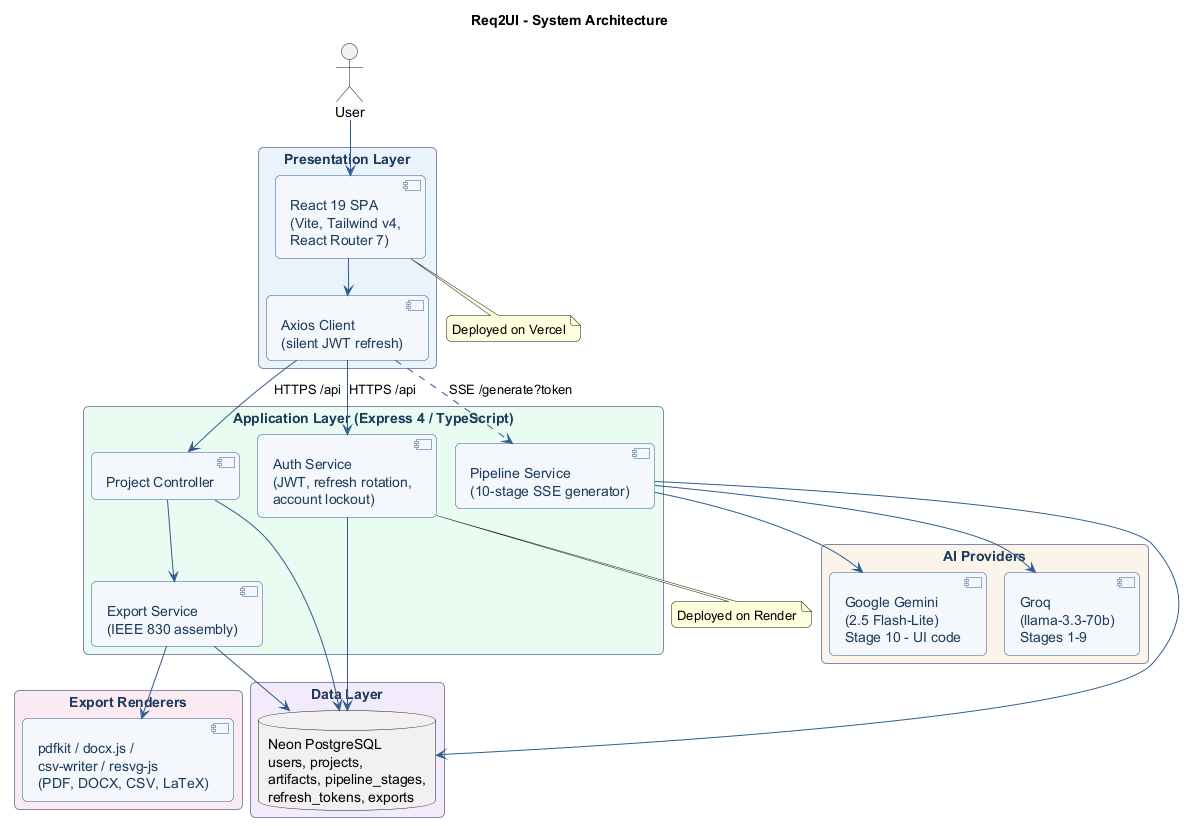
\includegraphics[width=\linewidth]{architecture.png}
  \caption{Architecture diagram}
  \label{fig:architecture}
\end{figure}

\subsection{System Context Diagram}
The Req2UI system operates as a central system that interacts with users, administrators, and external services. Users submit natural-language project descriptions and receive generated SRS documents, UI prototypes, and test cases. The system integrates with the Groq API for requirement and test-case generation, the Google Gemini API for UI code generation, and the OWASP Top 10 knowledge base for security analysis.

\begin{figure}[ht]
  \centering
  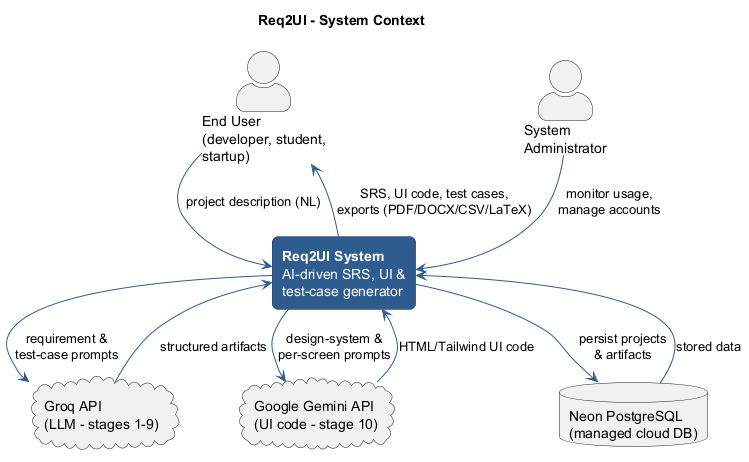
\includegraphics[width=0.95\linewidth]{context.png}
  \caption{System context diagram}
  \label{fig:context}
\end{figure}

\subsection{Class Diagram}
This class diagram shows the structural design of the system. The \texttt{Project} class is the central entity that groups all generated artifacts. Users can create multiple projects. Artifacts are typed (functional/non-functional/security requirements, test cases, wireframes, traceability, UML, and UI code). Service classes such as the Pipeline Service, Gemini Service, and Export Service operate on the project data but do not own it, ensuring separation of concerns and maintainability.

\begin{figure}[ht]
  \centering
  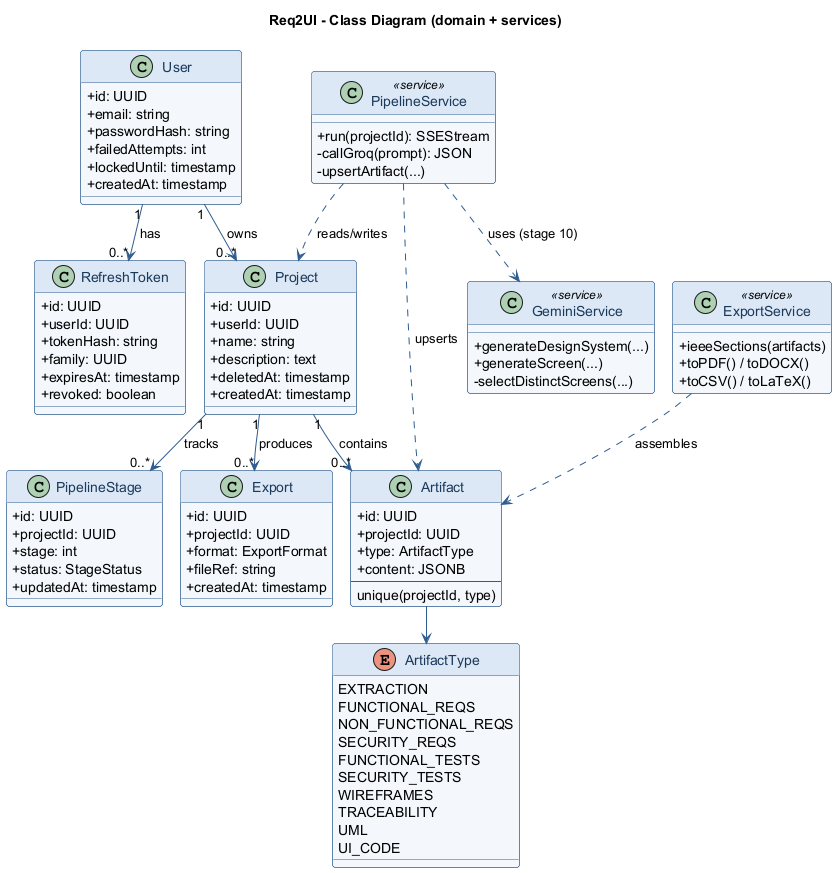
\includegraphics[width=\linewidth]{class.png}
  \caption{Class diagram}
  \label{fig:class}
\end{figure}

\subsection{Use Case Diagram}
The use case diagram captures the primary interactions between the End User and the system---registration/login, project management, artifact generation (which includes requirement, test-case, and UI-code generation), reviewing and refining artifacts, previewing UI code, and exporting---as well as the administrator's monitoring and user-management responsibilities.

\begin{figure}[ht]
  \centering
  
\includegraphics[width=\linewidth]{usecase.png}
  \caption{Use case diagram}
  \label{fig:usecase}
\end{figure}

\subsection{Sequence Diagram}
This sequence diagram describes the flow of interactions when a user generates artifacts. The request opens a Server-Sent Events (SSE) stream; the pipeline runs stages 1--9 against Groq, persisting each artifact and streaming progress, then runs stage 10 against Gemini to produce the design system and per-screen UI code before the artifacts viewer is rendered.

\begin{figure}[ht]
  \centering
  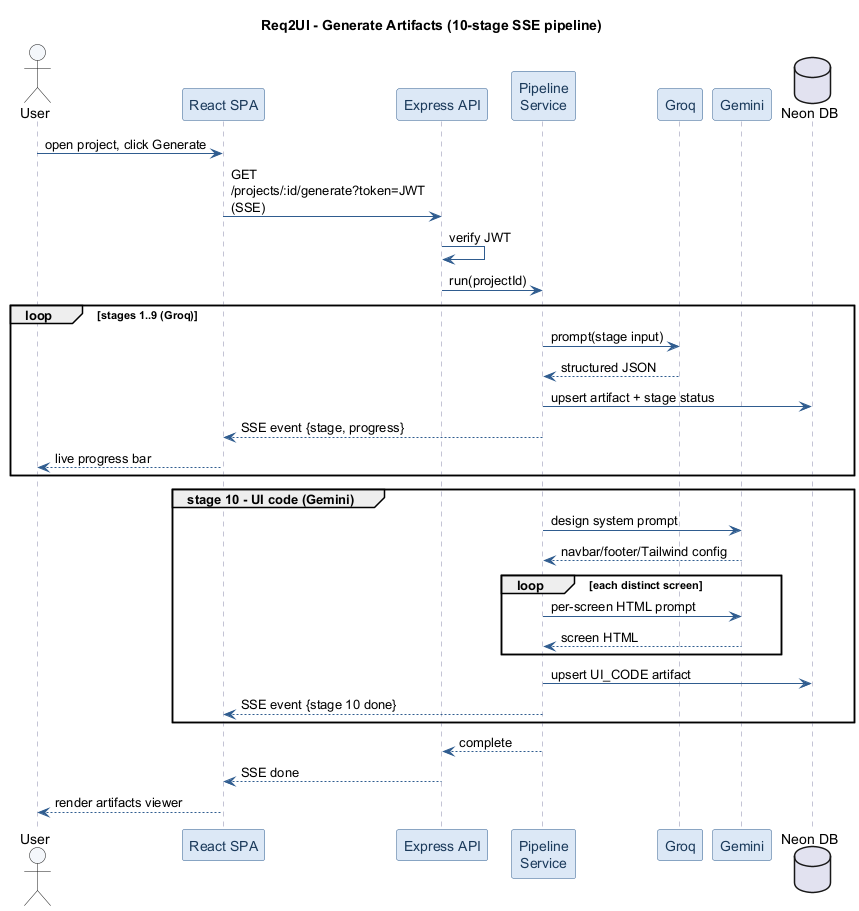
\includegraphics[width=\linewidth]{sequence.png}
  \caption{Sequence diagram}
  \label{fig:sequence}
\end{figure}

\subsection{Activity Diagram}
This activity diagram shows the end-to-end workflow of the system. It starts with user authentication and project setup, followed by input submission and validation. The pipeline then generates functional, non-functional, and security requirements, test cases, wireframes, UML, and UI code. Finally, the user reviews the results and exports the generated artifacts before returning to the dashboard.

\begin{figure}[ht]
  \centering
  
\includegraphics[width=0.85\linewidth]{activity.png}
  \caption{Activity diagram}
  \label{fig:activity}
\end{figure}

\section{Technologies and Tools Used}
\subsection{Non-Functional Testing and Evaluation Tools}
\begin{itemize}[leftmargin=*,nosep]
  \item \textbf{Apache JMeter:} evaluate system performance and response time.
  \item \textbf{Postman:} test API reliability and request--response behavior.
  \item \textbf{OWASP ZAP:} assess security requirements and common web vulnerabilities.
  \item \textbf{Hotjar / UserTesting:} evaluate usability and interaction efficiency.
  \item \textbf{UptimeRobot:} evaluate system availability and reliability.
\end{itemize}

\subsection{Implementation Technologies}
\begin{itemize}[leftmargin=*,nosep]
  \item \textbf{Frontend:} React 19, TypeScript, Tailwind CSS v4, Vite, React Router 7, Axios.
  \item \textbf{Backend:} Node.js, Express 4, TypeScript.
  \item \textbf{Database:} PostgreSQL via Neon (\texttt{@neondatabase/serverless}).
  \item \textbf{AI Providers:} Groq (\texttt{llama-3.3-70b-versatile}) for stages 1--9; Google Gemini 2.5 Flash-Lite for stage 10 (UI code).
  \item \textbf{Export:} pdfkit, docx.js, csv-writer, resvg-js (SVG$\rightarrow$PNG for diagram embedding).
  \item \textbf{Security:} OWASP Top 10 as the reference framework for security requirements and test cases.
  \item \textbf{Deployment:} Vercel (frontend) and Render (backend).
\end{itemize}

\section{Prototype}
The implemented web application provides the following primary screens, which constitute the working prototype:
\begin{itemize}[leftmargin=*,nosep]
  \item \textbf{Landing / Authentication} --- marketing landing page with registration and login forms.
  \item \textbf{Dashboard} --- lists the authenticated user's projects with status badges and entry points to create a new project.
  \item \textbf{Create Project} --- captures the project name and the natural-language description, with optional organization/document metadata and UI design preferences (theme, colour, navigation, density, etc.), plus worked example briefs that pre-fill a complete, detailed project.
  \item \textbf{Project Detail} --- shows the ten pipeline stages and streams live progress (via SSE) while generation runs.
  \item \textbf{Artifacts Viewer} --- displays the generated requirements, test cases, traceability matrix, and Mermaid-rendered UML diagrams, with export controls (PDF, DOCX, LaTeX, CSV).
  \item \textbf{UI Code Preview} --- renders the generated HTML screens in an embedded preview frame with navigation between screens, responsive (desktop/tablet/mobile) viewports, an instant accent-recolor control, and a panel for natural-language AI refinement of the generated UI.
\end{itemize}
% TODO: insert prototype screenshots of the above screens (captured from the running application).
\noindent\textit{Screenshots of the running application are inserted here.}

% ============================================================
\chapter{Implementation}
This chapter describes how the system was built: the implementation environment and stack, the database schema, the AI generation pipeline, the authentication and security model, the export subsystem, and the deployment topology.

\section{Implementation Environment}
The system is implemented as a full-stack \textbf{TypeScript} application split into two deployable units within a single repository.

\begin{itemize}[leftmargin=*,nosep]
  \item \textbf{Frontend:} React 19, Vite, Tailwind CSS v4, React Router 7, and Axios. It is a single-page application (SPA) that communicates with the backend over a REST API and an SSE stream.
  \item \textbf{Backend:} Node.js ($\geq$ 20) with Express 4, written in TypeScript and run with \texttt{ts-node-dev} in development. It exposes the REST API, the SSE generation endpoint, and the export endpoints.
  \item \textbf{Database:} PostgreSQL hosted on Neon, accessed through the \texttt{@neondatabase/serverless} driver.
  \item \textbf{AI providers:} Groq (\texttt{llama-3.3-70b-versatile}) for stages 1--9, and Google Gemini (\texttt{gemini-2.5-flash-lite}) for stage 10.
\end{itemize}

Configuration is supplied through environment variables (database URL, JWT secrets, Groq and Gemini API keys, and the frontend origin), validated at start-up before the server begins listening.

\section{Database Schema}
The schema comprises six tables, all using UUID primary keys and cascading foreign keys:
\begin{itemize}[leftmargin=*,nosep]
  \item \texttt{users} --- credentials and account-lockout fields (\texttt{failed\_attempts}, \texttt{locked\_until}).
  \item \texttt{refresh\_tokens} --- hashed refresh tokens with a \texttt{family} identifier and \texttt{revoked} flag for theft detection.
  \item \texttt{projects} --- user projects with a \texttt{status} field and soft-delete (\texttt{deleted\_at}).
  \item \texttt{artifacts} --- one JSONB \texttt{content} row per artifact type, with a \texttt{UNIQUE(project\_id, type)} constraint and a \texttt{version} counter that increments on every regeneration (upsert).
  \item \texttt{pipeline\_stages} --- per-stage status (\texttt{pending}/\texttt{running}/\texttt{completed}/\texttt{failed}), error text, and timestamps.
  \item \texttt{exports} --- references to generated export files.
\end{itemize}
The \texttt{UNIQUE(project\_id, type)} constraint is central to the resumable design: each stage performs an \texttt{INSERT \ldots\ ON CONFLICT DO UPDATE} so re-running the pipeline overwrites rather than duplicates artifacts.

\section{The AI Generation Pipeline}
The pipeline (Section~4.1.5) is implemented as a single orchestrator that drives ten stages. Each stage sends a system prompt (defining a strict JSON output schema) and a user prompt (the project context) to the LLM, then validates and persists the result.

\subsection{Structured Prompting and Robust Parsing}
Every Groq stage requests \texttt{response\_format: json\_object} at a low temperature (0.3) for deterministic, parseable output. The client guards against two failure modes: (i) on a length-truncated response it appends a ``be more concise'' instruction and retries with a smaller target; and (ii) transient errors and rate limits (HTTP 429) are retried with exponential backoff. A floor check after stage 2 aborts the run with an actionable message if fewer than three functional requirements could be derived, preventing a hollow SRS from vague input.

\subsection{Concurrency and Resumability}
Stages are grouped into dependency layers and the independent stages in each layer run concurrently (stages 3--5, then 6--7, then 8--10), shortening end-to-end latency. Before running, the orchestrator loads all existing artifacts for the project; any stage whose artifact is already present is marked complete and skipped, so an interrupted or failed run resumes from the point of failure. An explicit ``re-generate'' clears this cache and redoes every stage.

\subsection{UML Diagram Generation}
Stage 9 emits three UML diagrams (use case, class, sequence) as Mermaid source, which the frontend renders client-side; the output is sanitised to strip code fences that would break rendering.

\subsection{UI Code Generation (Stage 10)}
Stage 10 is the most elaborate stage and is implemented as a two-pass process on Gemini, summarised in Figure~\ref{fig:uicode}. Before any model call, a categorisation heuristic (\texttt{selectDistinctScreens}) deduplicates near-identical screens (e.g.\ login vs.\ register) so generation effort is spent on genuinely different pages, capped at six.

\textbf{Pass one --- shared design system.} A single Gemini call produces, as structured JSON, a shared navbar and footer, the page \texttt{body} classes, a \emph{reusable component class kit} (canonical Tailwind class strings for buttons, inputs, labels, cards, badges, tables, and empty states), and a small set of realistic, domain-appropriate \emph{sample-data} records. The component kit and sample data are then threaded verbatim into every screen prompt, which is what keeps the generated pages visually consistent (identical buttons, cards, and tables) and makes the application feel connected (the same entities recur across screens) rather than a set of disconnected mock-ups.

\textbf{Pass two --- per-screen HTML.} For each distinct screen the orchestrator gathers the screen's required components and the functional requirements relevant to it, falling back to the top general requirements when no specific match is found so that no page is generated from an empty context. The assembled prompt combines the design system, the component kit, the shared sample data, an accent configuration script, and explicit rules for Lucide icons, accessibility (semantic landmarks, \texttt{aria} labels, label/input association, AA contrast), responsiveness, and loading/empty/error states. Screens are generated in concurrent batches of three.

\textbf{Deterministic theming.} The brand accent is owned by code rather than the model: a helper emits a Tailwind configuration that, by default, reproduces the standard \texttt{indigo} scale, but when the user supplies a custom primary colour it deterministically derives a full 50--900 scale from that hex and \emph{redefines} \texttt{indigo} to it (\texttt{buildAccentScale}). Because every generated page references the same \texttt{indigo-*} utilities, this single substitution recolours the whole application reliably, and it also enables an instant, client-side recolor in the preview (remapping the Tailwind config and a small set of CSS overrides) with no additional model call.

\textbf{Robustness.} Generated HTML is checked for completeness (\texttt{htmlLooksComplete}) to catch silent truncation at the output-token ceiling; a page that looks cut off is regenerated once with a larger token budget. Gemini calls are funnelled through a throttled queue (minimum $\approx$4.5\,s spacing) to stay within free-tier rate limits, and ``thinking'' tokens are disabled so the output budget is spent on the visible HTML.

\textbf{Post-generation refinement.} After generation, the user can refine the result through natural-language instructions scoped to a single page, several pages, or the entire design system; the refinement is staged as a pending artifact and previewed before being applied or discarded, so changes are never destructive. The same screen also offers ready-made style presets and the instant accent recolor described above.

\begin{figure}[ht]
  \centering
  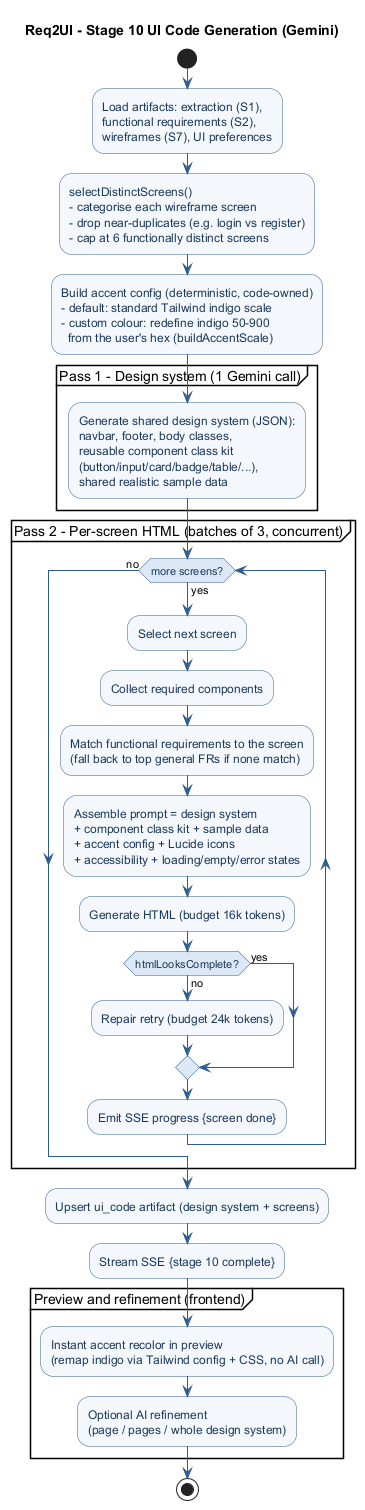
\includegraphics[height=0.92\textheight]{uicode.png}
  \caption{Stage 10 UI code generation: two-pass design-system and per-screen process with requirement grounding, deterministic theming, and output validation.}
  \label{fig:uicode}
\end{figure}

\section{Authentication and Security Implementation}
Authentication uses short-lived JWT access tokens (15 minutes) held in \texttt{sessionStorage} and long-lived refresh tokens (7 days) stored in an \texttt{httpOnly} cookie. Refresh tokens are SHA-256 hashed before storage and grouped into a \emph{family}; on each refresh the used token is rotated (revoked and replaced), and if an already-revoked token is presented the entire family is revoked --- a standard refresh-token-theft mitigation. Passwords are hashed with \texttt{bcrypt} (work factor 12). Five failed logins lock an account for 15 minutes. Additional hardening includes Helmet security headers, CORS restricted to the configured frontend origin with credentials, Zod schema validation on all auth inputs, an IP-based rate limiter (5 attempts per 15 minutes) on auth endpoints, and \texttt{trust proxy} configured for a single proxy hop so the rate limiter works correctly behind the hosting provider's proxy. The SSE generation endpoint accepts the access token as a query parameter because the \texttt{EventSource} API cannot set authorization headers.

\section{Export Subsystem}
Generated artifacts are assembled into an IEEE 830 document structure (\texttt{ieeeSections}) and rendered to four formats: \textbf{PDF} (pdfkit, with a styled title page, running headers/footers, colour-headed tables, and Mermaid diagrams rasterised to PNG via resvg-js), \textbf{DOCX} (docx.js with heading styles), \textbf{LaTeX} (a thesis-styled \texttt{report} with \texttt{xltabular} tables, compilable with pdfLaTeX), and \textbf{CSV} (a flat export of requirements, test cases, and the traceability matrix).

\section{Results and Discussion}
The implemented system successfully realises the full pipeline envisioned in the objectives: from a single natural-language description it produces functional, non-functional, and OWASP-aligned security requirements; functional and security test cases; a traceability matrix; UML diagrams; and runnable UI code --- all exportable in four formats. The resumable, concurrent pipeline makes generation both faster and resilient to transient LLM failures, and the streaming UI gives users live feedback during a multi-minute generation. The principal practical constraint encountered was LLM rate limiting (particularly Gemini's free tier), which is mitigated through request throttling, backoff, and the resume mechanism rather than eliminated.

% ============================================================
\chapter{Testing}
Testing the system spans two complementary levels: (i) the artifacts the system \emph{generates} for a user's project (the functional and security test cases produced by stages 5 and 6, documented in IEEE 829 form), and (ii) the verification of the platform itself through an automated unit/integration test suite. This chapter focuses on the latter, together with the evaluation strategy for the non-functional requirements.

\section{Automated Test Suite}
The backend is covered by a Jest test suite executed with \texttt{npm test} (\texttt{jest --runInBand}). The suite mocks the database and token service so routes are tested in isolation, and uses \texttt{supertest} to drive the Express application. At the time of writing, the suite comprises \textbf{nine test suites and 94 passing tests}.

\begin{longtable}{L{3.4cm} L{1.4cm} L{8cm}}
\caption{Automated test coverage}\\
\toprule
\textbf{Suite} & \textbf{Tests} & \textbf{What is verified} \\
\midrule
\endhead
Authentication routes & 9 & Registration validation (missing fields, short password), duplicate-email rejection (409), successful registration (201 + access token), login with valid/invalid credentials, non-existent user, and logout cookie clearing. \\
Auth middleware & 4 & Rejection of missing/invalid/expired bearer tokens and acceptance of a valid token with the decoded user attached to the request. \\
Project routes & 9 & Project create/list/read/soft-delete, ownership enforcement, validation of name/description bounds, and optional metadata and UI-preference payloads. \\
Token service & 8 & Refresh-token issuance, SHA-256 hashing, rotation, family-based revocation on reuse, and expiry handling. \\
Pipeline service & 4 & Orchestration flow, stage sequencing, and resumability (skipping stages whose artifact already exists). \\
Pipeline helpers & 26 & Screen categorisation, distinct-screen selection (dedup/backfill/limit), Mermaid sanitisation, deterministic accent-scale construction, the indigo-remap accent config, and HTML completeness validation. \\
Metrics service & 12 & Coverage and traceability metric calculations over requirements and test cases. \\
UI preferences & 7 & Mapping of preference fields to prompt guidance, custom-colour handling, and omission of empty/``AI-chooses'' values. \\
Export service & 15 & LaTeX document structure (title page, front matter, numbered chapters), colour palette and styled headings, requirement tables, balanced \texttt{xltabular}/\texttt{itemize}/\texttt{enumerate} environments, folding of acceptance criteria and controls into rows, and CSV header/row correctness and counts. \\
\bottomrule
\end{longtable}

\section{Functional and Security Test Cases (IEEE 829)}
For each generated project, the system itself produces functional test cases (stage 5; at least two per functional requirement, including positive and negative paths) and security test cases (stage 6; attack-vector-driven, one or more per security requirement). These are presented to the user in IEEE 829 form---identifier, coverage link, preconditions, steps, and expected result---and are exported in the PDF, DOCX, and CSV documents. The traceability matrix (stage 8) then quantifies coverage, reporting the proportion of functional requirements linked to test cases.

\section{Non-Functional Evaluation}
The non-functional requirements (Section~4.3) are evaluated with the tools identified there: Apache JMeter / Locust for response time and load, Postman / k6 for API latency, axe / WAVE for accessibility, and UptimeRobot / Pingdom for availability monitoring of the deployed services. % TODO: insert measured results (response-time distributions, concurrent-user load test, accessibility audit) once the evaluation runs are completed.

\section{Security Validation}
Beyond the generated security test cases, the platform's own security posture is validated against the OWASP Top 10 controls implemented in Chapter~6: bcrypt password hashing, JWT validation, refresh-token rotation with family-based theft detection, account lockout, input validation (Zod), rate limiting, security headers (Helmet), and TLS in transit. % TODO: attach OWASP ZAP / Burp Suite scan results for the deployed environment.

% ============================================================
\chapter{Conclusion and Future Work}
\section{Conclusion}
This project set out to reduce the manual effort, inconsistency, and security oversights inherent in early-stage software documentation by automating it end-to-end. The delivered system, Req2UI, takes a single natural-language project description and, through a ten-stage AI pipeline, produces a complete IEEE 830 Software Requirements Specification---functional, non-functional, and OWASP Top 10--aligned security requirements---together with IEEE 829 functional and security test cases, a requirements traceability matrix, UML diagrams, and runnable HTML/Tailwind UI code, all exportable as PDF, DOCX, LaTeX, and CSV.

Measured against the objectives in Section~1.3, the project met each one: an AI system that generates complete SRS documents automatically; integrated, context-driven security requirement generation; requirement-driven UI prototype generation; automated functional and security test-case generation; and a workflow that brings security and testing concerns forward to the requirements phase. The integrated pipeline directly addresses the research gap identified in Chapter~3---the absence of a single tool spanning natural-language input through SRS, UI prototype, and security-aware test cases with end-to-end traceability.

\section{Limitations}
The system's output quality is bounded by the underlying language models and by the detail of the user's input; vague descriptions yield thinner specifications, which the pipeline detects and reports rather than masks. Generation latency and throughput are constrained by third-party API rate limits, particularly on free tiers, and the generated UI code is intended as a low-fidelity prototype rather than a finished application. Non-functional targets such as concurrent-user load and full WCAG~2.1~AA conformance are specified but require dedicated evaluation runs to confirm.

\section{Future Work}
Promising extensions include: an administrative dashboard for usage monitoring and user management; extending the natural-language refinement already available for the UI artifact to the textual artifacts (requirements and test cases); iterative refinement loops where the model critiques and improves its own output without user prompting; export to additional formats and direct integration with issue trackers and design tools; fine-tuning or retrieval augmentation on domain-specific requirements corpora to improve accuracy; broadening the security analysis beyond the OWASP Top 10 to standards such as ASVS; and automated execution of the generated functional test cases against the generated UI.

% ============================================================
\begin{thebibliography}{9}
\bibitem{ref1} O. Matsuura et al., ``Automatic generation of web-based UI prototypes from UML requirements models.'' Available: \url{https://www.jstage.jst.go.jp/article/jssst/27/2/27_2_2_14/_article}
\bibitem{ref2} R. Khankhoje, ``An In-Depth Review of Test Automation Frameworks: Types and Trade-offs.''
\bibitem{ref3} B. Wei, ``Requirements are All You Need: From Requirements to Code with LLMs,'' 2023.
\bibitem{ref4} S. K. T. Pushparaj et al., ``A survey on automatic test case generation.'' Available: \url{https://www.ijtrd.com/papers/IJTRD5488.pdf}
\bibitem{ref5} A. Fatima et al., ``NLP-based test case generation,'' Journal of Computing \& Biomedical Informatics, 2025.
\bibitem{ref6} A. Goknil et al., ``Automatic Generation of System Test Cases from Use Case Specifications,'' 2015.
\bibitem{ref7} R. Batool et al., ``Automated Categorization of Software Security Requirements,'' 2025.
\end{thebibliography}

% ============================================================
\appendix
\chapter{Senior Project Summary Report}
\textbf{Project Title:} Req2UI: From Natural Language to Secure Software Artifacts Using AI.

\noindent\textbf{Supervisor:} Dr. Salma Radwan Abdel-Hamid.

\noindent\textbf{Team members:}
\begin{itemize}[leftmargin=*,nosep]
  \item Mennatallah Hany Mohamed Attia --- 221007653
  \item Mayar Hany Mohamed Attia --- 221007654
  \item Malak Tarek Farouk Tolba --- 221007884
  \item Yasmin Haitham Shaheen --- 221017815
  \item Mohamed Bassem Emam --- 221027617
\end{itemize}

\noindent\textbf{Project Deliverables:} % TODO
\noindent\textbf{Local Impact:} % TODO
\noindent\textbf{Global Impact:} % TODO
\noindent\textbf{Team Organization:} % TODO
\noindent\textbf{Ethical Considerations:} % TODO
\noindent\textbf{Social Impact:} % TODO
\noindent\textbf{Professional Responsibility:} % TODO
\noindent\textbf{Standards:} IEEE 12207, IEEE 830, IEEE 829, UML, OWASP Top 10.
\noindent\textbf{Realistic Constraints:} deadline, budget, software, and hardware constraints (see Section~1.5).

\end{document}
